% \iffalse
\let\negmedspace\undefined
\let\negthickspace\undefined
\documentclass[beamer]{IEEEtran}
\usepackage{cite}
\usepackage{amsmath,amssymb,amsfonts,amsthm}
\usepackage{algorithmic}
\usepackage{graphicx}
\usepackage{textcomp}
\usepackage{xcolor}
\usepackage{txfonts}
\usepackage{listings}
\usepackage{enumitem}
\usepackage{mathtools}
\usepackage{gensymb}
\usepackage{comment}
\usepackage[breaklinks=true]{hyperref}
\usepackage{tkz-euclide} 
\usepackage{listings}
\usepackage{gvv}                                        
\def\inputGnumericTable{}                                 
\usepackage[latin1]{inputenc}                                
\usepackage{color}                                            
\usepackage{array}                                            
\usepackage{longtable}                                       
\usepackage{calc}                                             
\usepackage{multirow}                                         
\usepackage{hhline}                                           
\usepackage{ifthen}                                           
\usepackage{lscape}
\usepackage[export]{adjustbox}

\newtheorem{theorem}{Theorem}[section]
\newtheorem{problem}{Problem}
\newtheorem{proposition}{Proposition}[section]
\newtheorem{lemma}{Lemma}[section]
\newtheorem{corollary}[theorem]{Corollary}
\newtheorem{example}{Example}[section]
\newtheorem{definition}[problem]{Definition}
\newcommand{\BEQA}{\begin{eqnarray}}
\newcommand{\EEQA}{\end{eqnarray}}
\newcommand{\define}{\stackrel{\triangle}{=}}
\theoremstyle{remark}
\newtheorem{rem}{Remark}
\begin{document}
\parindent 0px
\bibliographystyle{IEEEtran}

\title{GATE - EC 27}
\author{EE23BTECH11215 - Penmetsa Srikar Varma$^{}$% <-this % stops a space
}
\maketitle
\newpage
\bigskip

\renewcommand{\thefigure}{\theenumi}
\renewcommand{\thetable}{\theenumi}
\section*{Question}
Q27) Let m\brak{\text{t}} be a strictly band-limited signal with bandwidth B and energy E. Assuming $\omega_0$ = 10B, the energy in the signal $\text{m}\brak{\text{t}}\text{cos}\brak{\omega_0\text{t}}$\\[1ex]
\brak{\text{A}}\ $\frac{\text{E}}{4}$\\[1ex]
\brak{\text{B}}\ $\frac{\text{E}}{2}$\\[1ex]
\brak{\text{C}}\ \text{E}\\[1ex]
\brak{\text{D}}\ 2\text{E} \qquad\qquad\qquad\quad\qquad\qquad\qquad\qquad\brak{\text{GATE EC 2023}}
\section*{Solution}
\begin{table}[h]
    \centering
    \begin{tabular}{|c|c|c} 
    \hline
        Variables & Conditions \\
    \hline
        M\brak{\text{f}} & Fourier transform of m\brak{\text{t}}\\
    \hline
         \text{y}\brak{\text{t}} & \text{y}\brak{\text{t}}=$\text{m}\brak{\text{t}}\text{cos}\brak{2\pi\text{f}_0\text{t}}$\\
    \hline
        Y\brak{\text{f}} & Fourier transform of y\brak{\text{t}}\\
    \hline
    \end{tabular}

    \label{tab:my_label}
\end{table}
\begin{center}
    Table of Parameters\\[5ex]
\end{center}

\begin{figure}[h]
    \centering
    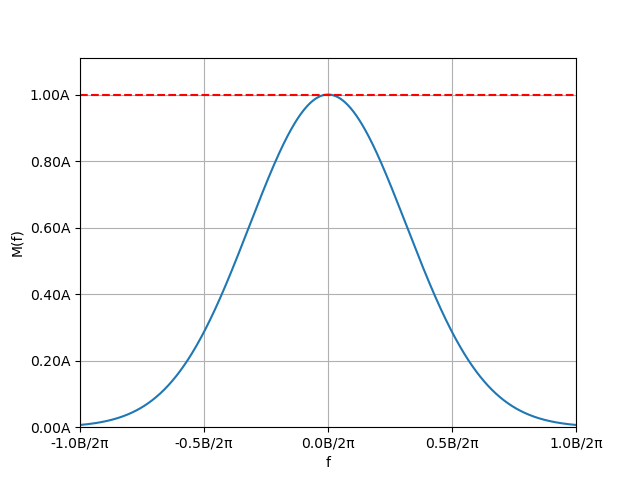
\includegraphics[scale=0.50]{figs/ec,27.png}
    \label{fig:enter-label}
\end{figure}

Energy \brak{\text{E}} of the signal m\brak{\text{t}} is given by,
\begin{align}
    \text{E}&=\int_{-\infty}^{\infty}|\text{m\brak{\text{t}}}|^2\ \text{dt}
\end{align}
According to Parseval's theorem,
\begin{align}
\label{2}
    \text{E}&=\int_{-\infty}^{\infty}|\text{M}\brak{\text{f}}|^2\text{df}\ \propto\ \text{A}^2
\end{align}
Fourier transform of y\brak{\text{t}} is given by,
\begin{align}
\text{Y\brak{\text{f}}}&=\text{M\brak{\text{f}}}*\frac{1}{2}\brak{\delta\brak{\text{f}_0+\text{f}}+\delta\brak{\text{f}-\text{f}_0}}
\end{align}
We have $\text{f}_0$=$\frac{10}{2\pi}$B,
\begin{align}
\text{Y\brak{\text{f}}}&=
\begin{cases}
    \frac{\text{M\brak{\text{f}}}}{2}&\frac{9\text{B}}{2\pi}\leq\abs{\text{f}}\leq\frac{12\text{B}}{2\pi}\\
    0 & \text{otherwise}
\end{cases}
\end{align}
\begin{figure}[h]
    \centering
    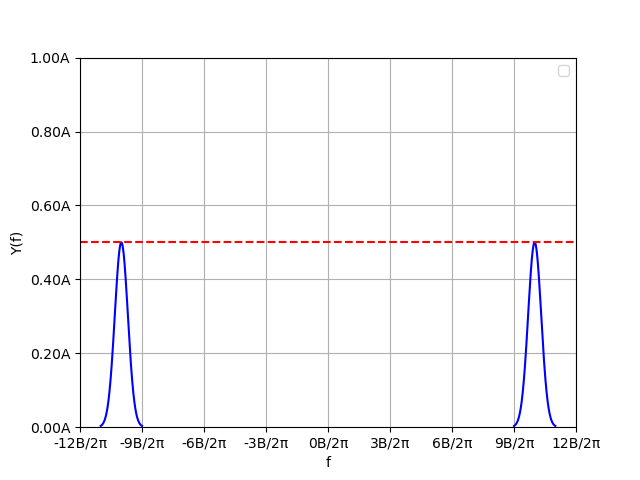
\includegraphics[scale=0.50]{figs/ec,27(1).png}
    \label{fig:enter-label}
\end{figure}

Energy $\brak{\text{E}_1}$ of the signal y\brak{\text{t}} is given by sum of energies of individual bandwidth signals,

\begin{align}\text{E}_1\propto \brak{\frac{\text{A}}{2}}^2+\brak{\frac{\text{A}}{2}}^2=\frac{\text{A}^2}{2}\end{align}
from \brak{\ref{2}},\\
$$\text{E}_1=\frac{\text{E}}{2}$$
So, option B is correct
\end{document}
